\chapter{Describing fission using nuclear density functional theory}\label{chap:Model}

%(Nicolas gave a good annotated presentation in 2017 that describes some of the philosophy, as well as some of the outstanding challenges of spontaneous fission in an adiabatic framework: \verb|https://t2.lanl.gov/fiesta2017/school/Schunck_NotesSlides.pdf|)

There are basically two microscopic frameworks in which to study fission: time-dependent and static (time-independent). Since fission is an inherently time-dependent process, time-dependent methods offer deep insight into the fission process and the characteristics of the fragments, especially kinetic and excitation energies~\cite{Scamps2019, Scamps2015a, Simenel2014, Bulgac2016a, Umar2010}. However, they can only treat a single event at a time and are quite expensive, making them impractical for fission yield predictions. Furthermore, and most important to a discussion of spontaneous fission, is the fact that fully time-dependent approaches have no mechanism with which to describe quantum tunneling, making them totally unsuited to spontaneous fission calculations. Finally, even if the tunneling problem was solved, this approach would still be unsuitable for any nucleus with a reasonably-long lifetime (compared to a typical time step size ${\sim}10^{-22}$ sec).

In the other, so-called static approach, it is assumed that collective motion of the nucleus is slow compared to the intrinsic motion of the nucleons, and therefore that collective and intrinsic degrees of freedom can be decoupled. This assumption of adiabaticity is supported by experimental evidence which suggests a characteristic timescale for fission (from saddle to scission, the point at which the neck snaps) of ${\sim}10^{-20}-10^{-18}$sec, compared to typical nuclear timescales on the order of ${\sim}10^{-22}$sec (see~\cite{Jacquet2009} for a review of fission timescale experiments). The validity of the adiabatic assumption was further discussed for fission and other nuclear processes in~\cite{Nazarewicz1993}.

The assumption of adiabaticity justifies the creation of a potential energy surface (PES) in some space of collective shape coordinates, and the dynamics of fission are then described in terms of trajectories across the PES. Quantum tunneling pops out in a fairly natural way in this formalism using the WKB approximation, and half-life estimates follow. The kinetic and excitation energies can be computed in this framework, but they are extremely sensitive to the characterization of scission, which is not well-defined in static frameworks~\cite{Younes2011}. However, as we shall show, the static approach is well-suited to estimating fission yields.

%Adiabaticity: For fusion reactions, N,Z equilibrium reached in ${\sim}10^{-21}$ seconds, then energy/thermal equilibrium in a similar time scale, then finally mass equilibrium in ${\sim}10^{-19}$ - Yuri has a slide with these time scales from his talk Monday. By comparison, what is an appropriate timescale for collective motion? I suppose that is nucleus-dependent

In an effort to be as self-consistent as possible, the PES is computed in the framework of nuclear DFT, which combines the Hartree-Fock-Bogoliubov variational approximation to the energy with a many-body method inspired by Kohn-Sham DFT. An overview of this self-consistent mean-field framework is described below, followed by a description of the dynamical calculations which are used to calculate fission yields.

\section{Nuclear density functional theory}
As with all nonrelativistic quantum systems, nuclei can be described using the many-body Schr\"{o}dinger equation. However, one often finds this type of description difficult or impossible in practice, for two reasons:

\begin{itemize}
\item In order to use the Schr\"{o}dinger equation, one needs to describe the interactions between nucleons. However, protons and neutrons interact via the strong nuclear force, which is non-perturbative at low energies and has a complex spin and isospin dependence.% Owing to this, as well as to the fact that protons and neutrons are themselves made up of smaller particles, an analytic expression for the nucleon-nucleon interaction (analogous to the $\frac{1}{r}$ form of the Coulomb interaction) is not available.
\item Even if an interaction was known precisely, nuclei are large systems made up of many protons and neutrons. Solving the Schr\"{o}dinger equation directly quickly becomes computationally intractable as the number of particles increases.
\end{itemize}

Nuclear density functional theory is one of several methods which has been developed to address these challenges. It is particularly useful for heavy nuclei, where other approaches such as configuration interaction and \textit{ab initio} methods become prohibitively expensive.

\subsection{Density functional theory}\label{sect:DFT}
Nuclear DFT is rooted in the Hohenberg-Kohn theorems~\cite{Hohenberg1964}, which are briefly described in the following.

The first Hohenberg-Kohn theorem states that the energy of the system is a uniquely-defined functional $E(\rho)$ of the particle density $\rho(\vec{r})$. This means one can describe a complicated system of N interacting particles using a single density which depends on 3 coordinates, rather than many-body wavefunction depending on 3N coordinates - a huge simplification!

The second Hohenberg-Kohn theorem states that the functional which gives the energy of the system will give the ground state energy if, and only if, it acts on the true ground state density: $E(\rho)=E_{gs} \iff \rho = \rho_{gs}$. Thus, given a particular functional $E(\rho)$, one can vary the input density $\rho$ to minimize the total energy and be assured that one is approaching the ground state energy of the system. In the case of electronic systems, a variational prescription to compute the electron density was subsequently proposed by Kohn and Sham in~\cite{Kohn1965}. However, extensions of this prescription to nuclei, which are self-bound objects governed by a poorly-known Hamiltonian, led to a Kohn-Sham scheme that was too difficult to be applied~\cite{engel2007,barnea2007,messud2009}. Instead, the practical alternative is to introduce mean-field variational methods such as Hartree-Fock (HF) and Hartree-Fock-Bogoliubov (HFB), as we do in Section~\ref{sect:HFB}.

The next step is to find the correct energy density functional. Unfortunately, neither the Hohenberg-Kohn theorems nor the Kohn-Sham method specify how this is to be done. In anticipation of mean-field plus pairing methods such as HFB (see Section~\ref{sect:HFB}), the total energy will instead be assumed to be a sum of several contributions, each of which can be treated individually in terms of the particle density $\rho(\vec{r},\vec{r}')$:
\begin{equation}\label{eq:EDFterms}
E(\rho) = E_{kin} + E_{Coul} + E_{nuc} + E_{pair},
%E(\rho, \kappa) = \int d^3\vec{r}\sum_{t=0,1}\mathcal{H}_t = \int d^3\vec{r}\left(\mathcal{H}_{kin} + \mathcal{H}_{nuc} + \mathcal{H}_{Coul, dir} + \mathcal{H}_{Coul, exch} + \mathcal{H}_{pair}\right)
\end{equation}

\noindent where $E_{kin}$ is the kinetic energy term, $E_{Coul}$ comes from the Coulomb interaction between protons, $E_{nuc}$ is a nucleon-nucleon interaction term, and $E_{pair}$ describes the tendency of nucleons to form pairs, a behavior which would otherwise be smeared out in non-interacting mean-field models. Each of the terms in~\eqref{eq:EDFterms} is described below.

\subsubsection{Kinetic energy term}

Defining the kinetic density $\tau_\alpha = \left.\nabla\cdot\nabla'\rho_\alpha(\vec{r},\vec{r}')\right|_{\vec{r}=\vec{r}'}$, $\alpha=p,n$, the kinetic energy contribution is
\begin{equation}
E_{kin} = \frac{\hbar^2}{2m} \left(1-\frac{1}{A}\right) \int d^3\vec{r} \left(\tau_n(\vec{r}) + \tau_p(\vec{r}) \right),
\end{equation}

\noindent where $A$ is the number of nucleons and $m$ is the mass of a single nucleon. The $\left(1-\frac{1}{A}\right)$ term is a simple center-of-mass correction.

\subsubsection{Coulomb interaction term}
The repulsive Coulomb interaction between protons is divided into a direct term and an exchange term, which is related to the antisymmetry of proton wave functions:
\begin{align}
E_{Coul} &= E_{Coul, dir} + E_{Coul, exch}, \\
E_{Coul, dir}& = \frac{e^2}{2} \int d^3\vec{r}_1 d^3\vec{r}_2 \frac{\rho_p(\vec{r}_1)\rho_p(\vec{r}_2)}{\abs{\vec{r}_1-\vec{r}_2}}, \\
E_{Coul, exch} &= \frac{e^2}{2} \int d^3\vec{r}_1 d^3\vec{r}_2 \frac{\rho_p(\vec{r}_2,\vec{r}_1)\rho_p(\vec{r}_1,\vec{r}_2)}{\abs{\vec{r}_1-\vec{r}_2}}.
\end{align}

\noindent The direct term uses local densities, which are related to the nonlocal densities found in the exchange term: $\rho(\vec{r}) = \rho(\vec{r},\vec{r})$. Often, the exchange term is computed in the Slater approximation~\cite{Slater1951, TitinSchnaider1974}:
\begin{equation}
E_{Coul, exch} \approx -\frac{3e^2}{4} \left(\frac{3}{\pi}\right)^\frac{1}{3} \int d^3\vec{r} \rho_p^\frac{4}{3}(\vec{r}).
\end{equation}

\subsubsection{Nuclear interaction term}\label{sect:skyrmeterm}
Describing the interaction energy between nucleons $E_{nuc}$ (and to a lesser extent, $E_{pair}$) continues to be an active area of research in nuclear theory today~\cite{Machleidt2011,Machleidt2016,Epelbaum2009,Detmold2015,Stroberg2019}. For nuclear DFT, the most commonly-used strong-interaction energy density functionals belong to the Skyrme, Gogny, or covariant family of functionals (each of which is discussed in~\cite{bender2003}). We will primarily be using Skyrme functionals, which can be written as a sum of time-even and time-odd terms~\cite{Dobaczewski1995}:
\begin{align}
E_{Skyrme} &= \int d^3\vec{r} \sum_{t=0,1} \left( \mathcal{H}^{even}_t + \mathcal{H}^{odd}_t \right),\\
\mathcal{H}^{even}_t &= C^\rho_t\rho_t^2 + C_t^{\Delta\rho}\rho_t\Delta\rho_t + C^\tau_t\rho_t\tau_t + C^J_t\mathsf{J}^2_t + C^{\nabla J}_t\rho_t\nabla\cdot\vec{J}_t, \\
\mathcal{H}^{odd}_t &= C^s_t \vec{s}_t^2 + C_t^{\Delta s}\vec{s}_t\Delta\vec{s}_t + C^T_t\vec{s}_t\cdot\vec{T}_t + C^j_t\mathsf{j}^2_t + C^{\nabla j}_t\vec{s}_t\cdot(\nabla\times\vec{j}_t),
\end{align}

\noindent where $\tau_t$ is the kinetic energy density; $\mathsf{J}_t$ and $\vec{J}_{\kappa,t}$ are, respectively, the scalar and vector parts of the spin current density; $\vec{s}_t$ is the spin density; $\vec{T}_t$ is the spin kinetic density; and $\vec{j}_t$ is the momentum density (to see how these each relate to $\rho$, see e.g.~\cite{bender2003}). The index $t=0(1)$ refers to isoscalar(isovector) energy densities, e.g. $\rho_0 = \rho_n + \rho_p$ ($\rho_1 = \rho_n - \rho_p$). Note that $\mathcal{H}^{even}_t$ depends only on time-even densities (and similarly for $\mathcal{H}^{odd}_t$).

Since this energy density functional is phenomenological, rooted in a zero-range contact force between nucleons, the coefficients must be determined from experiment and/or \textit{ab initio} theory. There are dozens of Skyrme parameterizations on the market, each one optimized to a particular observable or set of observables. The parameter sets SkM*~\cite{Bartel1982} and UNEDF1~\cite{Kortelainen2012} (along with its derivative, {\hfb}~\cite{Schunck2015}) have been optimized to datasets which include fission data, making them suitable for fission calculations.

\subsubsection{Pairing interaction term}
The simplest mean field approximation fails to take into account some correlations between nucleons, especially correlations between nucleons which occupy nearby states. Such nucleons (for example, those occupying orbitals with equivalent orbital quantum numbers but opposite spins) have a tendency to form pairs, similar in mechanism to BCS superconductivity or $^3$He superfluidity~\cite{brink2005}. To help account for these correlations, we introduce a so-called pairing density $\kappa(\vec{r})=\kappa(r,\sigma,\tau)$ (which will be defined in Section~\ref{sect:HFB}) and use a density-dependent pairing functional~\cite{chasman1976}:
\begin{equation}
E_{pair} = \sum_{\alpha=p,n} V_\alpha \int d^3\vec{r} \left( 1-\left(\frac{\rho(\vec{r})}{\rho_0}\right)^\beta \right)f\left(\kappa(\vec{r})\right),
\end{equation}

\noindent where $f\left(\kappa(\vec{r})\right) = \sum_{\sigma\tau}\sigma^2\kappa_\alpha(r,\sigma\tau;r,-\sigma,\tau)\kappa_\alpha^*(r,\sigma\tau;r,-\sigma,\tau)$ connects states with opposite spins. As with the nuclear interaction term, the pairing term contains adjustable parameters $V_0, \beta,$ and $\rho_0$. The denominator $\rho_0$ determines whether pairing is concentrated within the volume ($\rho_0\rightarrow\infty$), around the surface ($\rho_0\approx0.16$ fm$^{-3}$), or somewhere in between. The exponent $\alpha$ can partially account for the formation of surface effects, such as neutron skins and halos, but is usually set to $\alpha=1$. The pairing strength $V_0$ may be adjusted to experimental odd-even mass differences.

\subsection{Hartree-Fock-Bogoliubov method}\label{sect:HFB}
\subsubsection{Kohn-Sham and Hartree-Fock methods}

Having now chosen an energy density functional, the variational principle is invoked to find the density which minimizes the total energy, approximating the ground state of the system. The Kohn-Sham variational method was proposed soon following the Hohenberg-Kohn theorems in \cite{Kohn1965}. Given the exact energy density functional, Kohn-Sham actually solves the many-body problem exactly; however, as stated before, its use in nuclear physics is limited, principally because nuclei are self-bound systems with no external constraining potential. Kohn-Sham has been extended to self-bound systems (for instance in~\cite{engel2007,barnea2007,messud2009}), but the resulting expressions are complicated and in practice it is common to fall back on a mean-field approximation, such as Hartree-Fock.

The Hartree-Fock method, which actually predates Kohn-Sham by over 30 years, treats the system as a set of independent particles, each interacting with a mean field created by the other particles~\cite{Ring1980}. The mean-field approximation is well-justified in nuclear physics, its primary experimental evidence being the existence of magic numbers. The downside to Hartree-Fock is that some correlations, such as pairing correlations, are lost. The Hartree-Fock-Bogoliubov method introduces pairing correlations in the following way.

\subsubsection{Bogoliubov transformation}

In anticipation of the HFB formalism, we define the so-called Bogoliubov transformation. The fundamental entities in the Bogoliubov transformed basis are `quasiparticle' states, defined by quasiparticle creation and annihilation operators given by
\begin{align}
\beta_\mu &= \sum_i U^*_{i\mu}c_i + \sum_i V^*_{i\mu}c_i^\dagger, \\
\beta_\mu^\dagger &= \sum_i U_{i\mu}c_i^\dagger + \sum_i V_{i\mu}c_i,
\end{align}

\noindent or in block matrix notation,

\begin{equation}
\left(\begin{array}{c} \beta \\ \beta^\dagger\end{array}\right) = 
\left(\begin{array}{cc} U^\dagger & V^\dagger \\ V^T & U^T \end{array}\right)
\left(\begin{array}{c} c \\ c^\dagger\end{array}\right)
\equiv \mathcal{W}^\dagger \left(\begin{array}{c} c \\ c^\dagger\end{array}\right),
\end{equation}

\noindent where $c_i^\dagger, c_i$ are single particle creation and annihilation operators, and where the transformation matrix $\mathcal{W}$ must be unitary to ensure that $\beta, \beta^\dagger$ obey the fermion commutation relations~\cite{Ring1980}. The HFB ground state $\ket{\Phi_0}$ is defined to be a quasiparticle vacuum, such that $\beta_\mu\ket{\Phi_0}=0$ for all $\mu$.

As before, the system is described using a density matrix, which can be written in terms of single particle operators and an HFB vacuum state: $\rho_{ij} = \expval{c_j^\dagger c_i}{\Phi_0}$. In the HFB case, one must also define a second density matrix, called the pairing density: $\kappa_{ij} = \expval{c_jc_i}{\Phi_0}$. %, which can be thought of as a coupling between a state with $N-2$ particles and a state with $N$ particles.
In coordinate space, the density matrix $\rho$ and the pair tensor $\kappa$ take the form
\begin{align}
\rho(\vec{r},\vec{r}') &= \expval{c_{\vec{r}'}^\dagger c_{\vec{r}}}{\Phi_0}, \\
\kappa(\vec{r},\vec{r}') &= \expval{c_{\vec{r}'} c_{\vec{r}}}{\Phi_0}.
\end{align}

\noindent The densities $\rho$ and $\kappa$ are combined to form a single HFB generalized density matrix:
\begin{equation}
\mathcal{R} = \left(\begin{array}{cc}
\rho & \kappa \\
-\kappa^* & 1-\rho^*
\end{array}\right).
\end{equation}

\noindent Note that in nuclei, there are two $\mathcal{R}$'s: one for describing neutrons and another for protons.
%In general, $E$ is a functional of the generalized density $\mathcal{R}$.

\subsubsection{HFB equations}

The ground state configuration of the system with a particular energy density functional is described by the density $\mathcal{R}$ which minimizes $E(\mathcal{R})$. The solution can be found through the variational principle, in which the energy is minimized with respect to the generalized density, subject to the constraint that $\mathcal{R}^2=\mathcal{R}$. Defining the HFB Hamiltonian density $\mathcal{H}_{ba} \equiv 2 \partial E/\partial \mathcal{R}_{ab}$, this variation leads to the expression $\left[\mathcal{H},\mathcal{R}\right]=0$, which is called the Hartree-Fock-Bogoliubov equation.

The HFB equation is not typically solved in its commutator form, but rather it is recast in the following way: Recalling that two Hermitian operators whose commutator is zero can be simultaneously diagonalized, we choose to diagonalize $\mathcal{H}$ using the same Bogoliubov transformation $\mathcal{W}$ which diagonalizes $\mathcal{R}$:
\begin{equation}
\mathcal{W}^\dagger \mathcal{H} \mathcal{W} \equiv \mathcal{E} \qquad\mathrm{or}\qquad \mathcal{H}\mathcal{W} = \mathcal{W}\mathcal{E},
\end{equation}

\noindent where
\begin{equation}
\mathcal{E} = \left(\begin{array}{cc}
E_\mu & 0 \\
0 & -E_\mu
\end{array}\right)
\end{equation}

\noindent is a matrix of quasiparticle energies. In this form, the problem can then be solved iteratively:
\begin{enumerate}
	\setlength\itemsep{-2em}
	\item Choose some ansatz to estimate the density;\\
	\item Construct the HFB Hamiltonian density $\mathcal{H}$;\\
	\item Solve the eigenvalue problem: $\mathcal{H}\mathcal{W} = \mathcal{W}\mathcal{E}$; \label{hfb_iteration}\\
	\item Extract the densities corresponding to the eigenfunctions (which are related to $\mathcal{W}$);\\
	\item Update $\mathcal{H}$; \\
	\item Repeat starting from~\ref{hfb_iteration} until some predetermined convergence criterion is met.
\end{enumerate}

% https://ocw.mit.edu/courses/physics/8-04-quantum-physics-i-spring-2013/study-materials/MIT8_04S13_OnCommEigenbas.pdf

Often one will want to minimize the energy of the system subject to a particular constraint. Constraints can be introduced via the method of Lagrange multipliers. Some common examples of constraints include multipole moments representing nuclear shape deformations. In this case, a particular multipole moment might be constrained to the value $\bar{Q}_{\lambda\mu}$:
\begin{equation}\label{eq:routhian}
E' = E - \sum_{\lambda\mu} C_{\lambda\mu} \left(\expval{\hat{Q}_{\lambda\mu}} - \bar{Q}_{\lambda\mu}\right)^2.
\end{equation}

\noindent Since the Bogoliubov transformation breaks particle number symmetry, an important constraint on average particle numbers represents the first step towards particle number restoration:
\begin{equation}
E' = E - \lambda_n \expval{\hat{N}_n} - \lambda_p \expval{\hat{N}_p},
\end{equation}

\noindent where $\lambda_\alpha$ is determined by the condition that $\expval{\hat{N}_\alpha} = N_\alpha$ (more sophisticated particle number restoration schemes also exist, such as the Lipkin-Nogami method~\cite{Stoitsov2007, Lipkin1960, Nogami1964, Pradhan1973, Flocard1997}). % Discuss PAV and VAP? Only if requested

The collective coordinates employed in this dissertation are described in the following table:


\begin{tabular}{|ccc|}
	\hline \textbf{Coordinate} & \textbf{Units} & \textbf{Description} \\ \hline
	$Q_{20}$ & b & Axial quadrupole moment \\
	& & Roughly corresponds to elongation \\
	$Q_{22}$ & b & Triaxial quadrupole moment \\
	$Q_{30}$ & b$^\frac{3}{2}$ & Axial octupole moment \\
	& & Roughly corresponds to mass asymmetry \\
	$\lambda_{2}$ & MeV & Dynamic pairing fluctuations \\ \hline
\end{tabular} 

\subsection{Nucleon localization function}\label{sect:locali}
The major advantage nuclear DFT offers over microscopic-macroscopic models is a direct link to the underlying many-body structure. This can be visualized using the nucleon localization function (NLF), originally introduced for the identification of localized electronic groups in atomic and molecular systems in~\cite{Becke1990} and then applied to nuclei in~\cite{Reinhard2011,Zhang2016}. The NLF is defined using the single particle densities $\rho, \tau$, and \textbf{j} from before in the following way (with q=isospin and $\sigma$=spin/signature quantum number):
\begin{equation}
\mathcal{C}_{q\sigma} = \left[1+\left(\frac{\tau_{q\sigma}\rho_{q\sigma}-\frac{1}{4}|\nabla\rho_{q\sigma}|^2-\mathbf{j}^2_{q\sigma}}{\rho_{q\sigma}\tau_{q\sigma}^{TF}}\right)^2\right],
\end{equation}

\noindent where $\tau_{q\sigma}^{TF}=\frac{3}{5}(6\pi^2)^\frac{2}{3}\rho_{q\sigma}^\frac{5}{3}$. A localization value $\mathcal{C} \approx 1$ means that nucleons are well-localized; that is, the probability of finding two nucleons of equal spin and isospin in the same spatial region is low. A value of $\mathcal{C}=\frac{1}{2}$ corresponds to a Fermi gas of nucleons, as found in nuclear matter.

\begin{figure}
	\centering
	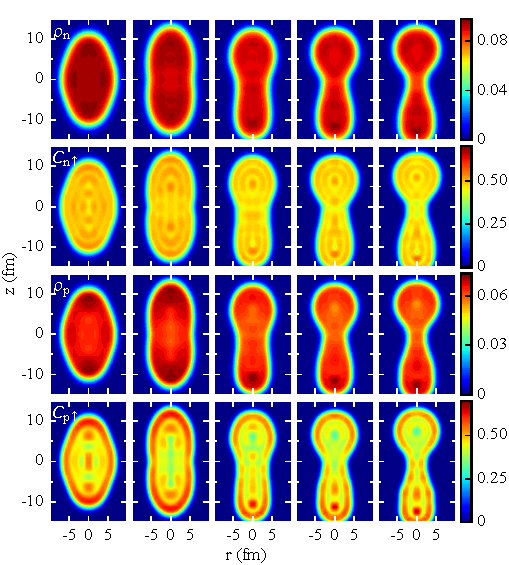
\includegraphics[width=0.5\linewidth]{TeX_files/methods_locali}
	\caption[Proton and neutron densities $\rho_p,\rho_n$ (in nucleons/fm$^3$) and spatial localizations $\mathcal{C}_p,\mathcal{C}_n$ for $^{240}$Pu at several configurations along the most-probable path to fission. Figure from~\cite{Zhang2016}.]{Proton and neutron densities $\rho_p,\rho_n$ (in nucleons/fm$^3$) and spatial localizations $\mathcal{C}_p,\mathcal{C}_n$ for $^{240}$Pu at several configurations along the most-probable path to fission. Figure from~\cite{Zhang2016}.}
	\label{fig:methodslocali}
\end{figure}

As demonstrated in Figure~\ref{fig:methodslocali}, the NLF tends to sharpen the internal structure of the nucleus compared to the density. When applied to fission as in~\cite{Sadhukhan2017}, it enables one to see the formation of well-defined prefragments whose shell structure is responsible for the peak of the fragment distribution.


\section{Microscopic description of nuclear fission}\label{sect:fissionmethod}
With a nuclear many-body method now in hand, it can be used as a tool to describe fission. Recently in~\cite{Sadhukhan2016}, a nuclear DFT-based approach based on this assumption was used to compute fragment yields from a PES that was computed self-consistently, using the WKB approximation to describe tunneling and Langevin dynamics to describe post-tunneling dissipation. The half-life can be computed as in~\cite{Sadhukhan2013}. The entire procedure, illustrated schematically in Figure~\ref{fig:methodsoverview}, is described below.

\begin{figure}
	\centering
	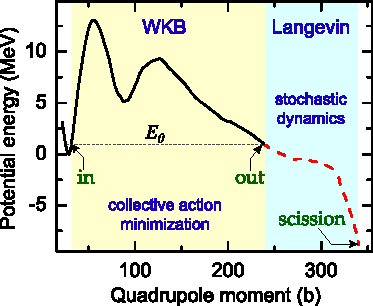
\includegraphics[width=0.5\linewidth]{TeX_files/methods_overview}
	\caption[Schematic overview of the Langevin framework for fission calculations used in this dissertation]{Schematic overview of the Langevin framework for fission calculations used in this dissertation. Figure from~\cite{Sadhukhan2016}.}
	\label{fig:methodsoverview}
\end{figure}

\subsection{Potential energy surfaces}
The primary degrees of freedom in the adiabatic approximation are nuclear collective shapes, and the basic ingredient to fission calculations is a PES. One could describe any nuclear configuration using a sufficiently-detailed PES; however, for practical computations one must use a truncated set of only a few collective coordinates. Thus, an important challenge for researchers is to select the most relevant collective coordinates, ideally while demonstrating that others can be safely neglected. Often, one will use the first few lowest-order moments, but there is some discussion within the community about whether these are the best for describing configurations on the way to fission, especially near scission (see, for instance,~\cite{younes2012}). Other collective coordinates which are sometimes used in the literature include $q_N=e^{-\frac{(\vec{r}-\vec{r}_{neck})^2}{a^2}}$, which is related to the size of the neck ($a=1$ fm is a common value for the range parameter), and non-geometric variables which control pairing and pairing fluctuations, such as the pairing gap $\Delta$ or the mean value of particle number fluctuations $\left\langle \Delta \hat{N}^2 \right\rangle$.

Once the appropriate collective-coordinate constraints $\vec{q}\equiv(q_1, q_2, \dots)$ are chosen, the PES is computed on a mesh: one DFT calculation per grid point. The density at each point $\vec{q}$ is then used to compute the HFB energy $E'(\vec{q})$~\eqref{eq:routhian}.

\subsection{Collective inertia}
Just as important as potential energy to the fission dynamics is the collective inertia, which describes the tendency of the system to resist configuration changes (such as shape changes)~\cite{Hill1953}. The form of the collective inertia used here is the non-perturbative adiabatic time-dependent HFB (ATDHFB) inertia with cranking~\cite{Baran2011}, which takes the form
\begin{equation}\label{eq:mATDHFB-np}
\mathsf{M}_{\mu\nu} =  \frac{\hbar^2}{2}\frac{1}{(E_a+E_b)}\left(\frac{\partial\mathcal{R}^{21}_{(0),ab}}{\partial q_\mu}\frac{\partial\mathcal{R}^{12}_{(0),ba}}{\partial q_\nu}+\frac{\partial\mathcal{R}^{12}_{(0),ab}}{\partial q_\mu}\frac{\partial\mathcal{R}^{21}_{(0),ba}}{\partial q_\mu}\right),
\end{equation}

\noindent The subscripts and superscripts are explained in the full temperature-dependent derivation of the collective inertia found in Appendix~\ref{append:TD-ATDHFB}, but an important feature to note is that computing the inertia requires differentiating the density matrix with respect to a pair of collective coordinates. In expressions where the collective coordinates are shape degrees of freedom, the collective inertia acts as a masslike term to resist changes to the collective motion.

A perturbative expression for the ATDHFB inertia also exists, which allows one to estimate the inertia without taking derivatives of the density~\cite{Baran2011}. It is computationally much faster and easier to implement, but it loses many of the important features of the inertia compared to the non-perturbative case, as we shall see in Chapter~\ref{chap:294Og}. Nevertheless, it is commonly-used in calculations and later on we shall show how this choice affects fission yields compared to the non-perturbative inertia.

Another common expression for the collective inertia comes from the Generator Coordinate Method (GCM). The GCM inertia also exists in two varieties: perturbative and non-perturbative~\cite{giuliani2018b}. Like the ATDHFB inertia, the perturbative GCM inertia is smoothed-out compared to the non-perturbative inertia. Both the perturbative and non-perturbative GCM inertias are found to be smaller in magnitude than their ATDHFB counterparts~\cite{Fiolhais1983,giuliani2018b}.

\subsection{WKB approximation}\label{sect:wkb}
Spontaneous fission is an extreme case of quantum tunneling. If the wave function of the fissioning nucleus is assumed to be slowly varying inside the (large) potential barrier (which condition is satisfied under the adiabatic assumption), then the WKB approximation allows us to estimate the probability of tunneling through a classically-forbidden region in the PES.

Under the WKB approximation, the most-probable tunneling path $\left. L(s) \right|_{s_{\rm in}}^{s_{\rm out}}$ in the collective space is found via minimization of the collective action
\begin{equation}\label{eq:action} 
S(L) = \frac{1}{\hbar}\int_{s_{\rm in}}^{s_{\rm out}} \sqrt{2\mathcal{M}(s)\left(E'(s)-E_0\right)}ds,
\end{equation} 

\noindent where $s$ is the curvilinear coordinate along the path $L$, $\mathcal{M}(s)$ is the effective collective inertia given by~\cite{Sadhukhan2013}
\begin{equation}
\mathcal{M}(s) = \sum_{\mu\nu} \mathsf{M}_{\mu\nu} \frac{dq_\mu}{ds} \frac{dq_\nu}{ds}
\end{equation}

\noindent and $E'(s)$ is the potential energy along $L(s)$. $E_0$ stands for the collective ground-state energy. The calculation is repeated for different outer turning points, and each of these points is then assigned an exit probability $P(s_{\rm out})=[1+\exp{2S(L)}]^{-1}$~\cite{Baran1978}. 

The half-life corresponds to the pathway of minimum action, and the expression for the half-life is $T_{1/2} = \mathrm{ln}(2)/nP(s_\mathrm{min})$, where the parameter $n$ is the number of assaults on the fission barrier per unit time and which we set to the standard value $n=\frac{1 \mathrm{MeV}}{h}\approx10^{20.38} s^{-1}$~\cite{Baran1978}. However, because of the exponential dependence of the half-life on the action, half-life calculations suffer from large uncertainties due to the uncertainties in theoretical ingredients.

\subsection{Langevin dynamics}

Although the link between collective and intrinsic degrees of freedom was assumed away in the adiabatic approximation, it is necessary to reintroduce some connection between the two, especially in the region between the outer turning points and scission where the adiabatic assumption is weakest. Through the semiclassical Langevin approach~\cite{Kubo1966}, we introduce a dissipation tensor $\eta$ that mimics energy exchange between intrinsic and collective modes. The dissipation tensor is related to a random force with strength $g$ via the fluctuation-dissipation theorem~\cite{Callen1951,Kubo1966}: $\sum_k g_{ik}g_{jk} = \eta_{ij}k_BT$. The fluctuation-dissipation theorem effectively couples collective and intrinsic degrees of freedom via the system temperature $T$, given by $k_BT = \sqrt{E^*/a}$ where $a=A/10$MeV$^{-1}$ parameterizes the level density and the excitation energy is given by $E^*(\vec{q}) = E'(s_{out}) - E'(\vec{q}) - \frac{1}{2}\sum\left(\mathcal{M}^{-1}\right)_{ij}p_i p_j$ (see~\cite{Abe1996,Frobrich1998,Sadhukhan2016} for details).

After emerging from the classically-forbidden region of the PES, fission trajectories proceed across the PES from the outer turning line, evolving according to the Langevin equations:
\begin{gather}\label{eq:langevin} 
	\frac{dp_i}{dt} =  
	-\frac{p_j p_k}{2} \frac{\partial}{\partial q_i}\left(\mathcal{M}^{-1}\right)_{jk} 
	- \frac{\partial E'}{\partial q_i}  - \eta_{ij}\left(\mathcal{M}^{-1}\right)_{jk} p_k + g_{ij}\Gamma_j(t) \,, \\ 
	\frac{dq_i}{dt} = 	\left(\mathcal{M}^{-1}\right)_{ij} p_j \,,  
\end{gather} 
\noindent where $p_i$ is the collective momentum conjugate to $q_i$, and $\Gamma_j(t)$ is a Gaussian-distributed, time-dependent stochastic variable. From here one can see that the dissipation term\\\noindent $- \eta_{ij}\left(\mathcal{M}^{-1}\right)_{jk} p_k$ represents a transfer of energy from the collective motion of the system to intrinsic single particle degrees of freedom, while the random fluctuation term $g_{ij}\Gamma_j(t)$ does the opposite.

Dissipation is treated in our work phenomenologically, since a self-consistent description of dissipation has not yet been fully developed~\cite{Bulgac2018a}.  In the meantime, we use the values of the dissipation tensor from~\cite{Sadhukhan2016}, which were fitted to reproduce the $^{240}$Pu spontaneous fission fragment yields.% However, work along this line has been started (maybe?) in refs 291-293 of~\cite{Schmidt2018} (see Section 4.1.1 for the context).

\subsection{Fragment identification via localization function}\label{sect:FragID}
The Langevin approach represents the best of what static approaches currently have to offer in terms of quantitative reproduction of the yields; however, it can be expensive and time-consuming to perform a full Langevin calculation with non-perturbative collective inertia in a multidimensional collective space. For applications where the level of quantitative accuracy is somewhat flexible (an example would be r-process network calculations, which are explained in Chapter~\ref{chap:rprocess}), one might ask whether it is necessary to do all these calculations if simple predictions are required (e.g., most-probable fission yields), or if there is some kind of physical insight that can be leveraged to reduce the workload.

By studying nucleon localization functions (Section~\ref{sect:locali}) for deformed configurations of fissioning nuclei, we observe that, in many cases, two distinct fragments start to form independently and then separate well before scission is reached (see Figure~\ref{fig:methodslocali}, taken from~\cite{Zhang2016}, as well as Sections~\ref{sect:178Ptfrags} and~\ref{sect:294Ogfrags}). Thus, a fissioning nucleus can be thought of as two well-formed prefragments connected by a neck. At scission, the two prefragments separate and the remaining neck nucleons are distributed to either of the two prefragments in some predictable way. Based on this, we developed a prescription for identifying prefragments and then estimating fragment yields at the outer turning line, using a statistical technique based on the grand canonical ensemble. This prescription is described in Appendix~\ref{append:Fragments}.